\documentclass[12pt]{article}
\usepackage{tikz}
\usepackage{amsmath, amssymb, amsfonts}
\usepackage{color}

\begin{document}
% 绘制红心

\begin{tikzpicture}
    \draw[red, fill=red] (0, 0) .. controls (0, 0.75) and (-1.5, 1.00).. (-1.5, 2) arc (180:0:0.75) -- cycle;
    \draw[red, fill=red] (0, 0) .. controls (0, 0.75) and ( 1.5, 1.00).. ( 1.5, 2) arc (0:180:0.75) -- cycle;    
\end{tikzpicture}

\vspace{2cm}

%% 绘制张量网络图
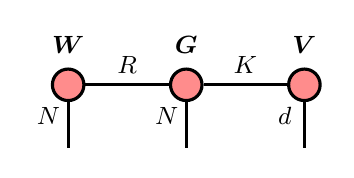
\begin{tikzpicture}
    % 1. 绘制三个圆形节点(W、G、V)
    \node [circle, % 节点形状:圆形
       line width=0.4mm, % 边框宽度
       draw=black, % 边框颜色
       fill=red!45, % 填充色:红色透明度45%
       inner sep=0pt, % 节点内部留白(设为0避免圆形变大)
       minimum size=0.4cm % 节点最小尺寸(固定圆形直径0.4cm)
      ] (w) at (0, 0) {}; % (w)是节点名称,(0,0)是坐标,{}内是节点内容为空
    \node at (0, 0.5) {\small{$\boldsymbol{W}$}}; % 在W节点上方0.5cm处标注W
    \node [circle, line width=0.4mm, draw=black, fill=red!45, inner sep=0pt, minimum size=0.4cm] (g) at (1.5, 0) {};
    \node at (1.5, 0.5) {\small{$\boldsymbol{G}$}}; 
    \node [circle, line width=0.4mm, draw=black, fill=red!45, inner sep=0pt, minimum size=0.4cm] (v) at (3, 0) {};
    \node at (3, 0.5) {\small{$\boldsymbol{V}$}}; 
    
    % 2. 绘制节点间的水平连线 + 标注
    \path [draw, line width=0.4mm, -] (w) edge (g); % W-G连线(无箭头)
    \node at (0.75, 0.25) {\small{$R$}}; % 连线上方标注R
    \path [draw, line width=0.4mm, -] (g) edge (v);
    \node at (2.25, 0.25) {\small{$K$}};

    % 3. 绘制节点向下的竖线 + 标注
    \draw [line width=0.4mm] (w) -- (0, -0.8);
    \node at (-0.25, -0.4) {\small{$N$}};
    \draw [line width=0.4mm] (g) -- (1.5, -0.8);
    \node at (1.5-0.25, -0.4) {\small{$N$}};
    \draw [line width=0.4mm] (v) -- (3, -0.8);
    \node at (3-0.25, -0.4) {\small{$d$}};
\end{tikzpicture}

\vspace{2cm}

%% ======= 网络张量图的优化代码 ===================== %% 
% 提升可读性和复用性
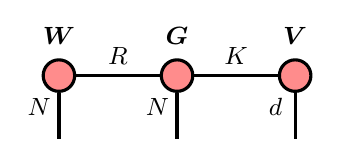
\begin{tikzpicture}[
    % 定义节点样式:复用性更强
    mynode/.style={circle, line width=0.4mm, draw=black, fill=red!45, inner sep=0pt, minimum size=0.4cm},
    myline/.style={line width=0.4mm},
    mylabel/.style={font=\small, inner sep=0pt}
]
    % 简化后的节点写法
    \node [mynode] (w) at (0, 0) {};
    \node [mylabel] at (0, 0.5) {$\boldsymbol{W}$};
    \node [mynode] (g) at (1.5, 0) {};
    \node [mylabel] at (1.5, 0.5) {$\boldsymbol{G}$};
    \node [mynode] (v) at (3, 0) {};
    \node [mylabel] at (3, 0.5) {$\boldsymbol{V}$};

    % 简化后的连线写法
    \path [myline] (w) edge (g);
    \node [mylabel] at (0.75, 0.25) {$R$};
    \path [myline] (g) edge (v);
    \node [mylabel] at (2.25, 0.25) {$K$};

    \draw [myline] (w) -- (0, -0.8);
    \node [mylabel] at (-0.25, -0.4) {$N$};
    \draw [myline] (g) -- (1.5, -0.8);
    \node [mylabel] at (1.25, -0.4) {$N$};
    \draw [myline] (v) -- (3, -0.8);
    \node [mylabel] at (2.75, -0.4) {$d$};
\end{tikzpicture}

\vspace{2cm}

% 减少重复代码、提升可维护性、增强扩展性、优化排版细节
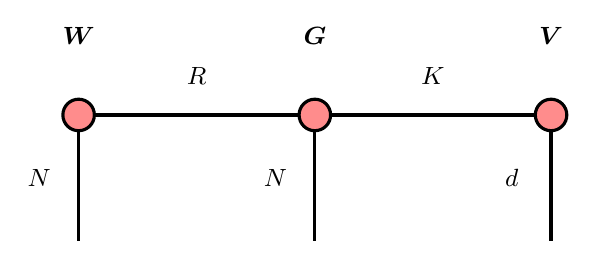
\begin{tikzpicture}[
    % 以下代码也可以放在导言区 \tikzset{}
    % 核心节点样式:参数化,方便统一修改
    mynode/.style={
        circle, % 节点形状:圆形 
        line width=0.4mm, % 边框宽度
        draw=black, % 边框颜色
        fill=red!45, % 填充色:红色透明度45%
        inner sep=0pt, % 节点内部留白(设为0避免圆形变大)
        minimum size=0.4cm  % 节点最小尺寸(固定圆形直径0.4cm)
        },
    % 线条样式:统一管理宽度
    myline/.style={line width=0.4mm},
    % 标注样式:明确字体大小+数学环境(避免样式混乱)
    mylabel/.style={
        font=\small, % 替代单独的\small,样式更集中
        inner sep=0pt % 消除标注节点的默认留白
        },
    % scale: 缩放, xscale: 横向缩放, yscale: 纵向缩放
    scale = 2
    ]
    % ========== 第一步:批量定义节点(减少重复坐标书写) ==========
    % 用\foreach循环批量创建核心节点,避免重复写\node
    \foreach \name/\label/\x in {w/W/0, g/G/1.5, v/V/3} {
        \node [mynode] (\name) at (\x, 0) {}; % 圆形节点
        \node [mylabel] at (\x, 0.5) {$\boldsymbol{\label}$}; % 上方标注
    }
    % ========== 第二步:批量绘制水平连线+标注 ==========
    \foreach \start/\end/\label/\x in {w/g/R/0.75, g/v/K/2.25} {
        \path [myline] (\start) edge (\end); % 水平连线
        \node [mylabel] at (\x, 0.25) {$\label$}; % 连线标注
    }
    % ========== 第三步:批量绘制竖线+标注 ==========
    \foreach \name/\label/\x in {w/N/-0.25, g/N/1.25, v/d/2.75} {
        \draw [myline] (\name) -- (\name |- 0, -0.8); % 竖线坐标复用
        \node [mylabel] at (\x, -0.4) {$\label$}; % 竖线标注
    }
\end{tikzpicture}



\end{document}